%*****************************************
\chapter{Tables}\label{ch05:tables}
%*****************************************

Excel workbooks are designed to store data and it is challenging to organize that data to yield meaningful information. Excel has many features that can help organize data and find needed information efficiently. Setting up data as a table from the onset allows users to sort, filter, total, and subtotal the data easily. In Excel, a table is a collection of data about a subject stored in adjacent rows and columns. Tables can improve the look and feel of a worksheet. This chapter explores how to set up, edit, and work with Excel tables effectively. These skills will be demonstrated in the context of a multi-sheet file that shows national average weather for two vastly different cities in the United States. Weather data is often voluminous and difficult to summarize since so much is collected every hour of every day and providing meaningful summaries of such data is a useful skill. The skills learned using weather data in this chapter can be transferred to data found in any discipline or field.

\section{Basic Table Skills}

\begin{center}
	\begin{objbox}{Learning Objectives}
		\begin{itemize}
			\setlength{\itemsep}{0pt}
			\setlength{\parskip}{0pt}
			\setlength{\parsep}{0pt}
			
			\item Understand table structure.
			\item Plan, create, and edit a table.
			\item Freeze rows and columns.
			\item Sort data in a table.
		\end{itemize}
	\end{objbox}
\end{center}

This section reviews the fundamental skills for setting up and maintaining an Excel table. The objective used for this chapter is the construction of a multi-sheet file to keep track of two cities' national weather data for the month of January. Organizing, maintaining, and reporting data are essentials skills for employees in most industries.

Figure \ref{05:fig01} shows the completed workbook that will be created in this chapter. Notice that this workbook contains four worksheets. The first worksheet contains weather data for Portland, Maine, the second contains weather data for Portland, Oregon, the third organizes the Oregon data by week, and the fourth contains subtotals for the Oregon data.

\begin{figure}[H]
	\centering
	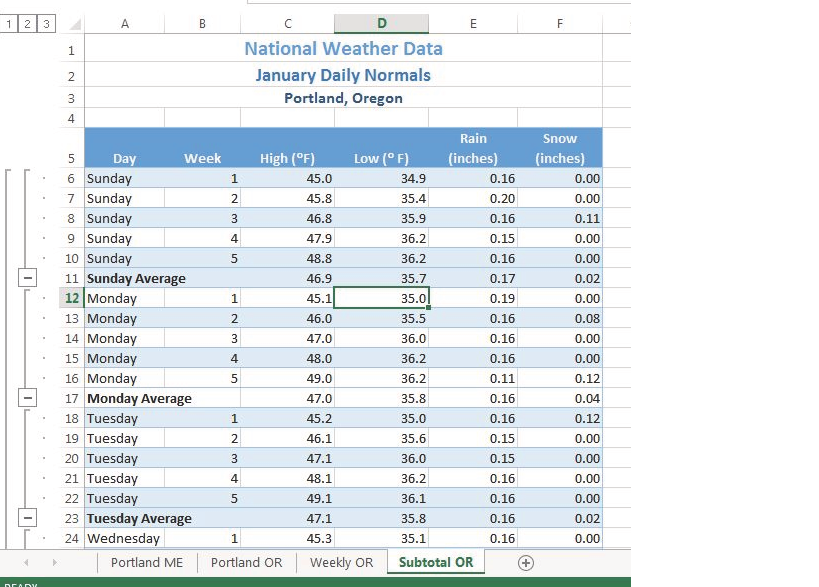
\includegraphics[width=\maxwidth{.95\linewidth}]{gfx/ch05_fig01}
	\caption{Completed National Weather Workbook}
	\label{05:fig01}
\end{figure}

\subsection{Creating a Table}

When data is presented in long lists or columns, it helps if the table is set up properly. Here are some rules of data-entry etiquette to follow when creating a table from scratch.

\begin{enumerate}
	\item Whenever possible, organize information using adjacent (neighboring) columns and rows.
	\item Start the table in the upper-left corner of the worksheet and work down the sheet.
	\item Do not skip columns and rows just to ``space out'' the information. To place white space between information in adjacent columns and rows, widen columns, heighten rows, or change the alignment.
	\item Reserve a single column at the left edge of the table for the table's row headings or identifying information.
	\item Reserve a single row at the top of the table for the table's column headings.
	\item If the table requires a title, put the title in the row(s) above the column headings.
\end{enumerate}

Following these rules will help ensure that the sorts, filters, totals, and subtotals applied to the table with return the desired results. With these rules in mind, begin working on \textit{National Weather} workbook. 

\begin{enumerate}
%fileopen CH5-Data
%filesave CH5-National Weather
	\item Open data file \fmtWorksheet{CH5-Data} and save the file as \fmtWorksheet{CH5-National Weather}.
	\item Click the \fmtWorksheet{Portland ME} worksheet tab to activate it.
	\item Notice that the data is in adjacent columns and rows. The upper-left corner of the table is in \fmtLoc{A5} and the titles are above the column headings in \fmtLoc{Row 5}.
	\item Click cell \fmtLoc{A5}.
	\item Click \fmtButton{Insert $ \Rightarrow $ Tables $ \Rightarrow $ Table}.
\end{enumerate}

The dialog box illustrated in Figure \ref{05:fig02} pops up. Excel has correctly determined that the data range is $ A5 $:$ E33 $ and that the table has headers.

\begin{figure}[H]
	\centering
	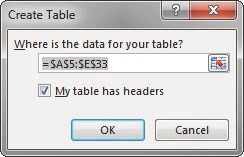
\includegraphics[width=\maxwidth{.95\linewidth}]{gfx/ch05_fig02}
	\caption{Create Table}
	\label{05:fig02}
\end{figure}

\begin{enumerate}[resume]
	\item Click \fmtButton{OK}.
	\item Click \fmtLoc{A5}.
	\item Adjust all column widths so that the complete headings are visible in \fmtLoc{Row 5} with the filter arrows showing. The filter arrows are the down-arrow buttons that appear in the header row when the table is created. 
\end{enumerate}

After this, the top of the worksheet will look like Figure \ref{05:fig03}.

\begin{figure}[H]
	\centering
	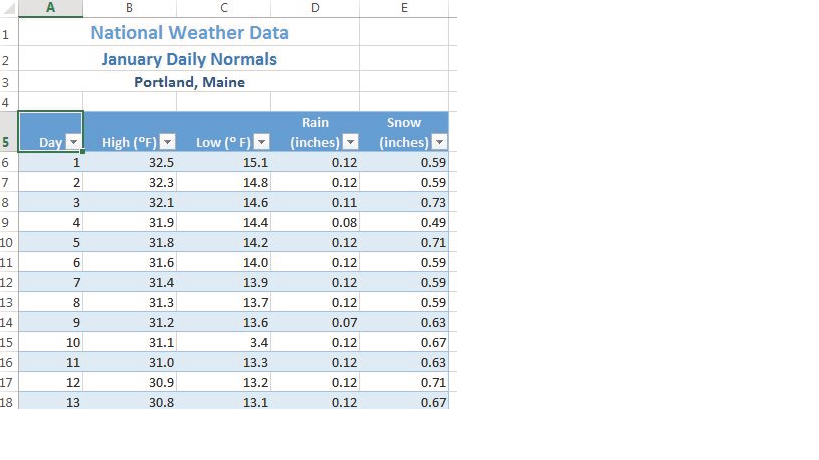
\includegraphics[width=\maxwidth{.95\linewidth}]{gfx/ch05_fig03}
	\caption{Weather Table}
	\label{05:fig03}
\end{figure}

Notice that a new ribbon tab, \textit{Table Tools Design}, appears when the mouse is clicked inside the table. This ribbon tab contains controls to edit, style, and add functionality to the table. (\fmtNewExcel{Excel 365}. The tab is named \textit{Table Design}, not \textit{Table Tools Design}.)

\begin{enumerate}
	\item Click the \fmtWorksheet{Portland OR} worksheet tab to activate it.
	\item Click cell \fmtLoc{A5}.
	\item Click \fmtButton{Insert $ \Rightarrow $ Tables $ \Rightarrow $ Table}.
	\item Be sure Excel automatically determines the data is in \fmtLoc{A5:E33} and that it has headers.
	\item Click \fmtButton{OK}.
	\item Click \fmtLoc{A5}.
	\item Adjust all column widths so that the complete headings are visible in \fmtLoc{Row 5} with the filter arrows showing. 
\end{enumerate}

\begin{center}
	\begin{sklbox}{Skill Refresher}
		\textbf{Create a Table}
		\\
		\begin{itemize}
			\setlength{\itemsep}{0pt}
			\setlength{\parskip}{0pt}
			\setlength{\parsep}{0pt}

			\item Click on the top left cell in the data.
			\item Click \textit{Insert $ \Rightarrow $ Tables $ \Rightarrow $ Table}.
			\item Make sure the data range is properly identified and \textit{My table has headers} is checked.
			\item Click \textit{OK}.
			\item Click on the top left cell again.
			\item Adjust all columns widths so the complete headings with the filter arrows are showing.
						
		\end{itemize}
	\end{sklbox}
\end{center}

\subsection{Formatting Tables}

There are many ways to format an Excel table. One of the easiest to use is a preset \textit{Table Style} using Light, Medium, or Dark colors. There are also a variety of \textit{Table Style Options} as listed in Table \ref{05:tab01}.

\begin{table}[H]
	\rowcolors{1}{}{tablerow} % zebra striping background
	{\small
		%\fontsize{8}{10} \selectfont %Replace small for special font size
		\begin{longtable}{L{1.0in}L{3.00in}} %Left-aligned, Max width: 4.25in
			\textbf{Table Style} & \textbf{Description} \endhead
			\hline
			Header Row & Top row of the table that includes column headings\\
			Total Row & Row added to the bottom that applies column summary calculations\\
			First Column & Formatting added to the left-most column in the table\\
			Last Column & Formatting added to the right-most column in the table\\
			Banded Rows & Alternating rows of color added to make it easier to see rows of data\\
			Banded Columns & Alternating columns of color added to make it easier to see columns of data\\
			Filter Button & Button that appear at the top of each column that lists options for sorting and filtering\\
			\rowcolor{captionwhite}
			\caption{Table Style Options}
			\label{05:tab01}
		\end{longtable}
	} % End small
\end{table}

Add formatting to both of the Portland weather tables in the following steps.

\begin{enumerate}
	\item Click on the \fmtWorksheet{Portland ME} sheet to activate it.
	\item Click cell \fmtLoc{A5}.
	\item Click \fmtButton{Table Tools Design $ \Rightarrow $ Table Styles $ \Rightarrow $ More Down Arrow}. (\fmtNewExcel{Excel 365}. The tab is named \textit{Table Design}, not \textit{Table Tools Design}.)
\end{enumerate}

A gallery of table styles will appear as in Figure \ref{05:fig04}.

\begin{figure}[H]
	\centering
	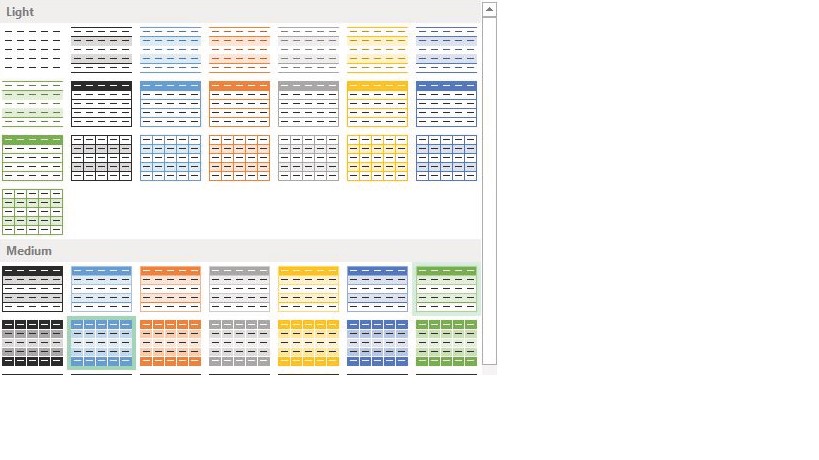
\includegraphics[width=\maxwidth{.75\linewidth}]{gfx/ch05_fig04}
	\caption{Table Styles}
	\label{05:fig04}
\end{figure}

\begin{enumerate}[resume]
	\item In the Table Styles gallery, in the Medium Section, click \textit{Table Style Medium} $ 7 $ (this is a green-colored style).
	\item Uncheck \fmtButton{Table Style Design $ \Rightarrow $ Table Style Options $ \Rightarrow $ Banded Rows}.
\end{enumerate}

The alternating colored rows will disappear. The data in the table is now more difficult to read.

\begin{enumerate}[resume]
	\item Try some of the other options in the Table Style Options group. When finished, be sure that \textit{Header Row}, \textit{Banded Rows}, and \textit{Filter Button} are the only ones checked, as in Figure \ref{05:fig05}.
	\item Save the \fmtWorksheet{CH5-National Weather} workbook.
\end{enumerate}

\begin{figure}[H]
	\centering
	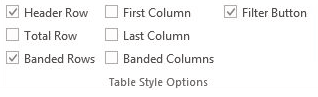
\includegraphics[width=\maxwidth{.65\linewidth}]{gfx/ch05_fig05}
	\caption{Ribbon Table Style Options}
	\label{05:fig05}
\end{figure}

\subsection{Adding Data to Tables}

Over time, new data will need to be added to a table, and that should be added in a blank row. The easiest way to do this is to enter the data below the last row in the table, then sort the table to arrange its data. If data must be added in a specific place in the middle of a table, insert a blank row and add the data there.

Add the last three days of the months to the \textit{Portland ME} and \textit{Portland OR} worksheets. The following steps walks through this process.

\begin{enumerate}
	\item Click on the \fmtWorksheet{Portland ME} worksheet.
	\item Click on \fmtLoc{A34} (the left-most cell below the last row in the table).
	\item Enter the data from the following table.
\end{enumerate}

\begin{table}[H]
	\rowcolors{1}{}{tablerow} % zebra striping background
	{\small
		%\fontsize{8}{10} \selectfont %Replace small for special font size
		\begin{longtable}{R{0.50in}R{0.50in}R{0.50in}R{0.50in}R{0.50in}} %Left-aligned, Max width: 4.25in
			\textbf{Day} & \textbf{High} (\textdegree F) & \textbf{Low} (\textdegree F) & \textbf{Rain} (inches) & \textbf{Snow} (inches) \endhead
			\hline
			$ 29 $ & $ 31.4 $ & $ 13.3 $ & $ 0.12 $ & $ 0.59 $ \\ 
			$ 30 $ & $ 31.6 $ & $ 3.4  $ & $ 0.08 $ & $ 0.47 $ \\ 
			$ 31 $ & $ 31.7 $ & $ 13.5 $ & $ 0.12 $ & $ 0.63 $ \\ 
			\rowcolor{captionwhite}
			\caption{Portland, Maine data}
			\label{05:tab02}
		\end{longtable}
	} % End small
\end{table}

Notice that the banded row formatting continues as additional rows are added to the tables.

\begin{enumerate}
	\item Click on the \fmtWorksheet{Portland OR} worksheet.
	\item Click on \fmtLoc{A34} (the left-most cell below the last row in the table).
	\item Enter the data from the following table.
\end{enumerate}

\begin{table}[H]
	\rowcolors{1}{}{tablerow} % zebra striping background
	{\small
		%\fontsize{8}{10} \selectfont %Replace small for special font size
		\begin{longtable}{R{0.50in}R{0.50in}R{0.50in}R{0.50in}R{0.50in}} %Left-aligned, Max width: 4.25in
			\textbf{Day} & \textbf{High} (\textdegree F) & \textbf{Low} (\textdegree F) & \textbf{Rain} (inches) & \textbf{Snow} (inches) \endhead
			\hline
			$ 29 $ & $ 48.8 $ & $ 36.2 $ & $ 0.16 $ & $ 0.00 $ \\ 
			$ 30 $ & $ 49.0 $ & $ 36.2 $ & $ 0.11 $ & $ 0.32 $ \\ 
			$ 31 $ & $ 49.1 $ & $ 36.1 $ & $ 0.16 $ & $ 0.00 $ \\ 
			\rowcolor{captionwhite}
			\caption{Portland, Oregon data}
			\label{05:tab03}
		\end{longtable}
	} % End small
\end{table}

\begin{enumerate}[resume]
%filesave CH5-National Weather	
	\item Save the \fmtWorksheet{CH5-National Weather} workbook.
\end{enumerate}

\subsection{Finding and Editing Data}

It is inevitable that data errors which need to be corrected will appear in a table. While it is possible to visually scan through a table to find errors, this can be a tedious and tiresome process, especially if the table is large. Excel can help with this through the \textit{Find} command. When using \textit{Find}, the best practice is to start with the cell pointer in cell $ A1 $ to ensure that all the data in the worksheet is included in the search.

A temperature of $ 3.4 $ degrees was entered erroneously in the \textit{Portland ME} sheet. It should have been $ 13.4 $. To fix this error, complete the following steps.

\begin{enumerate}
	\item Click on the \fmtWorksheet{Portland ME} sheet.
	\item Press the \fmtKeystroke{Ctrl}+\fmtKeystroke{Home} keys together to go to the top of the sheet (cell \fmtLoc{A1}).
	\item Click \fmtButton{Home $ \Rightarrow $ Editing $ \Rightarrow $ Find \& Select $ \Rightarrow $ Find}.
	\item In the \fmtButton{Find} box, type $ 3.4 $, and then click \fmtButton{Find Next}.
\end{enumerate}

\begin{figure}[H]
	\centering
	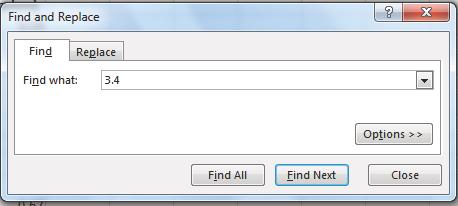
\includegraphics[width=\maxwidth{.95\linewidth}]{gfx/ch05_fig06}
	\caption{Find and Replace}
	\label{05:fig06}
\end{figure}

\begin{enumerate}
	\item Click the \fmtButton{Close} button.
	\item Replace $ 3.4 $ in the \textit{Low} column for Day $ 10 $ with $ 13.4 $.
	\item Now switch to the \fmtWorksheet{Portland OR} sheet and find the Snow error of $ 0.32 $ in Day $ 3 $. Change it to $ 0.12 $.
%filesave CH5-National Weather 
	\item Save the \fmtWorksheet{CH5-National Weather} workbook.
\end{enumerate}

\begin{center}
	\begin{sklbox}{Skill Refresher}
		\textbf{Finding and Replacing Data}
		\\
		\begin{itemize}
			\setlength{\itemsep}{0pt}
			\setlength{\parskip}{0pt}
			\setlength{\parsep}{0pt}

			\item Click \textit{Home $ \Rightarrow $ Editing $ \Rightarrow $ Find \& Select $ \Rightarrow $ Find}.
			\item In the \textit{Find} box, type the phrase to find then click \textit{Find Next}.
			\item Continue clicking \textit{Find Next} until the desired phrase is found.
			\item Click \textit{Close} and edit the data.
			
		\end{itemize}
	\end{sklbox}
\end{center}

\subsection{Freeze Rows and Columns}

When panes are ``frozen'' in a worksheet, Microsoft Excel keeps specific rows or columns visible in the table as it is scrolled on the screen. For example, if the first row in the spreadsheet contains labels, that row might be frozen to make sure that the column labels remain visible as the sheet is scrolled down. Follow these steps to freeze the worksheet headings and keep them visible on the screen.

\begin{enumerate}
	\item Click on the \fmtWorksheet{Portland ME} sheet.
	\item Click in \fmtLoc{A6}, the left-most cell \textit{below} the headings row.
	\item Click \fmtButton{View $ \Rightarrow $ Window $ \Rightarrow $ Freeze Panes $ \Rightarrow $ Freeze Panes} (see Figure \ref{05:fig07}).
	\item Scroll up and down the sheet and notice that the headings are always displayed at the top of the table. Also, notice that a thin line appears under \fmtLoc{Row 5} to mark the bottom of the frozen section.
\end{enumerate}

\begin{figure}[H]
	\centering
	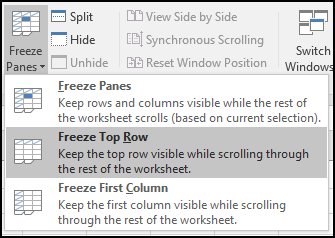
\includegraphics[width=\maxwidth{.65\linewidth}]{gfx/ch05_fig07}
	\caption{Freeze Pane}
	\label{05:fig07}
\end{figure}

To unfreeze the headings, follow these steps.

\begin{enumerate}

	\item Click \fmtButton{View $ \Rightarrow $ Window $ \Rightarrow $ Freeze Panes $ \Rightarrow $ Unfreeze Panes}

\end{enumerate}

\subsection{Simple Sort}

Content in a table can be sorted alphabetically, numerically, and in many other ways. Sorting helps organize data by ordering one or more columns in the table. Table \ref{05:tab04} describes the different sort orders available for each column of data.

\begin{table}[H]
	\rowcolors{1}{}{tablerow} % zebra striping background
	{\small
		%\fontsize{8}{10} \selectfont %Replace small for special font size
		\begin{longtable}{L{0.75in}L{1.00in}L{0.65in}L{1.50in}} %Left-aligned, Max width: 4.25in
			\textbf{Sort Order} & \textbf{Text} & \textbf{Numbers} & \textbf{Dates} \endhead
			\hline
			Ascending & Alphabetical (A-Z) & Smallest to Largest & Chronological (oldest to newest)\\
			Descending & Reverse Alphabetical (Z-A) & Largest to Smallest & Reverse Chronological (newest to oldest)\\
			\rowcolor{captionwhite}
			\caption{Sort Options}
			\label{05:tab04}
		\end{longtable}
	} % End small
\end{table}

Suppose it is important to know what the snowiest day was in January in Portland, Maine. One way to find that is to sort the \textit{Snow} column in Descending order.

\begin{enumerate}
	\item Click on the \fmtWorksheet{Portland ME} sheet.
	\item Click on the \fmtButton{Down Arrow} to the right of the header in \fmtLoc{E5}, \textit{Snow (inches)}.
	\item Click on Click \textit{ZA$ \downarrow $ Sort Largest to Smallest} (see Figure \ref{05:fig08}).
\end{enumerate}

\begin{figure}[H]
	\centering
	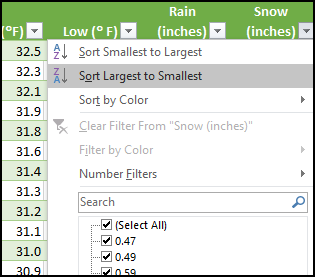
\includegraphics[width=\maxwidth{.65\linewidth}]{gfx/ch05_fig08}
	\caption{Sort by One Column}
	\label{05:fig08}
\end{figure}

If this is done correctly, the snowiest day, January 3rd (in \textit{Row} $ 6 $) with $ 0.73 $ inches of snow, will sort to the top of the list. Notice the filter arrow changes in the snow column to a downward pointing arrow to indicate that the column is sorted in descending order (largest to smallest).

\begin{figure}[H]
	\centering
	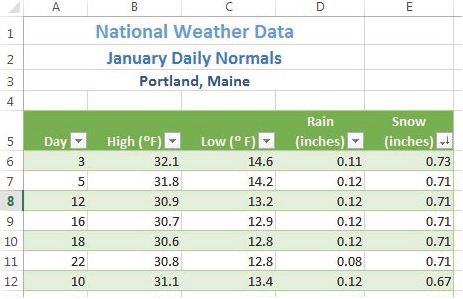
\includegraphics[width=\maxwidth{.95\linewidth}]{gfx/ch05_fig09}
	\caption{Snowiest Days in Maine}
	\label{05:fig09}
\end{figure}

\begin{enumerate}
	\item Now switch to the \fmtWorksheet{Portland OR} sheet and repeat these sort steps to find the snowiest day in Oregon. Check the worksheet with Figure \ref{05:fig10}.
\end{enumerate}

\begin{figure}[H]
	\centering
	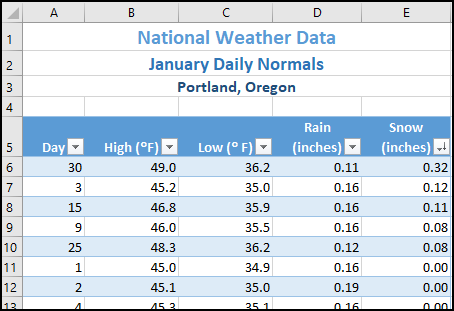
\includegraphics[width=\maxwidth{.95\linewidth}]{gfx/ch05_fig10}
	\caption{Snowiest Days in Oregon}
	\label{05:fig10}
\end{figure}

\begin{center}
	\begin{sklbox}{Skill Refresher}
		\textbf{Sort a Column}
		\\
		\begin{itemize}
			\setlength{\itemsep}{0pt}
			\setlength{\parskip}{0pt}
			\setlength{\parsep}{0pt}

			\item Click on the filter down arrow to the right of the header in the column to be sorted.
			\item Click on the choice \textit{AZ}$ \downarrow $ or \textit{ZA}$ \downarrow $ to sort the data in that column.
						
		\end{itemize}
	\end{sklbox}
\end{center}

\subsection{Multi-Level Sort}

Sometimes a table needs to be sorted by more than one column at a time to efficiently analyze the data. For example, if the data included different types of loans from several bank offices, it would need to be sorted by the type of loan and then by bank office name to clearly see the different groups of loans. As another example, if a worksheet included a list of grades for students over their time in high school, the data should be sorted first by student name, then by grade level (freshman, sophomore, junior, and senior) so that each student's grades appear in chronological order.

For the weather data, determine how cold the snow days were in Oregon.

\begin{enumerate}
	\item Click on the \fmtWorksheet{Portland OR} sheet.
	\item Click cell \fmtLoc{A6}.
	\item Click \fmtButton{Data $ \Rightarrow $ Sort \& Filter $ \Rightarrow $ Sort}.
	\item Click the down-arrow for \textit{Column Sort By} and select \textit{Snow (inches)}.
	\item Click the down-arrow for \textit{Order} and select \textit{Largest to Smallest}.
	\item To add a 2nd level sort, click \fmtButton{Add Level} at the top left corner of the dialog box.
	\item Click the down-arrow for \textit{Then by} and select \textit{Low (\textdegree F)}.
	\item In the same row, click the down-arrow for \textit{Order} and select \textit{Smallest to Largest}. The dialog box should look like Figure \ref{05:fig11}.
\end{enumerate}

\begin{figure}[H]
	\centering
	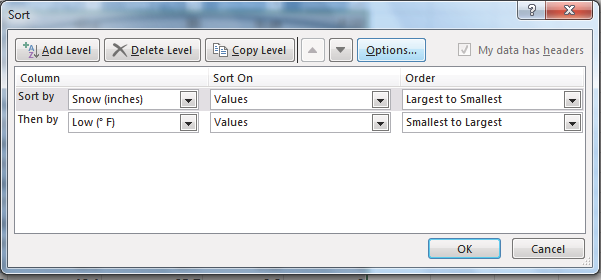
\includegraphics[width=\maxwidth{.95\linewidth}]{gfx/ch05_fig11}
	\caption{Multi-Level Sort}
	\label{05:fig11}
\end{figure}

\begin{enumerate}[resume]
	\item Click \fmtButton{OK}.
	\item The table sort results should look like Figure \ref{05:fig12}. Notice for the two days with $ 0.08 $ inches of snow, the low temp of $ 35.5 $ on Day $ 9 $ is displayed before the low temp of $ 36.2 $ on Day $ 25 $. The lowest of the two was listed first. Also notice that the filter arrows changed on the sorted columns to show how they are sorted.
\end{enumerate}

\begin{figure}[H]
	\centering
	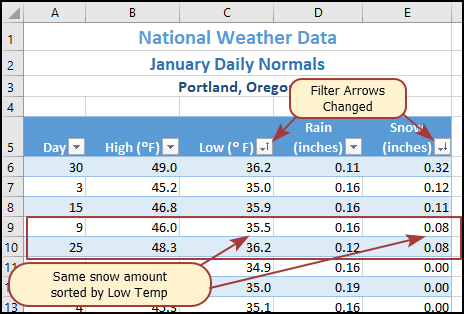
\includegraphics[width=\maxwidth{.95\linewidth}]{gfx/ch05_fig12}
	\caption{Multi-Level Sort Results}
	\label{05:fig12}
\end{figure}

\subsection{Custom Sorts}

In most cases, the data should be sorted in ``typical'' sort order: numbers sorted highest to lowest, words sorted alphabetically, etc. Some data does not make sense when sorted this way. For example, if the days of the week are sorted alphabetically, the result would be Friday, Monday, Saturday, Sunday, Thursday, Tuesday, and Wednesday. This order would be of no use to anyone! Similarly, the months of the year would not make sense alphabetically.

To illustrate how days can be sorted, a \textit{Week} number column was added to the \textit{Weekly OR} sheet. Then, the \textit{Day} column was changed from a number to names like Sunday. This sheet facilitates further analysis of the data to see if there are weekly trends in the weather. To look for those trends, sort the \textit{Weekly OR} sheet by \textit{Week} and then by \textit{Day}.

\begin{enumerate}
	\item Click on the \fmtWorksheet{Weekly OR} worksheet.
	\item Click cell \fmtLoc{A5}
	\item Click \fmtButton{Insert $ \Rightarrow $ Tables $ \Rightarrow $ Table}.
	\item Click \fmtButton{OK}.
	\item Click cell \fmtLoc{A5}.
	\item Click \fmtButton{Data $ \Rightarrow $ Sort \& Filter $ \Rightarrow $ Sort}	
	\item Click the down-arrow for \textit{Column Sort By} and select \textit{Week}.
	\item Click the down-arrow for \textit{Order} and select \textit{Smallest to Largest}.
	\item To add a 2nd level sort, click \fmtButton{Add Level} at the top left corner of the dialog box.
	\item Click the down-arrow for \textit{Then by} and select \textit{Day}.
	\item In the same row, click the down-arrow for \textit{Order} and select \textit{Custom List}. The dialog box should look like Figure \ref{05:fig13} will appear on the screen.
\end{enumerate}

\begin{figure}[H]
	\centering
	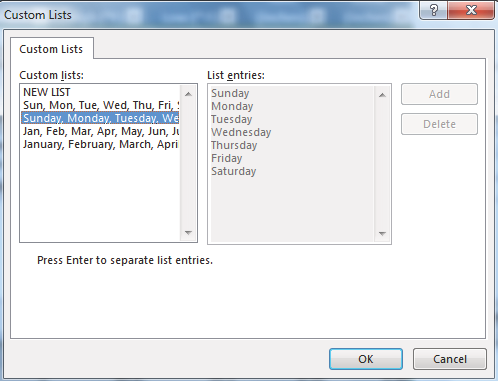
\includegraphics[width=\maxwidth{.95\linewidth}]{gfx/ch05_fig13}
	\caption{Custom Lists}
	\label{05:fig13}
\end{figure}

\begin{enumerate}[resume]
	\item Click on \fmtButton{Sunday, Monday, Tuesday, etc.} in the \textit{Custom} lists on the left-side of the dialog box. NOTE: Make sure to select the list with the days of the week spelled out, not the abbreviations for the days of the week.
	\item Click \fmtButton{OK}. 
	\item The \textit{Sort} dialog box should look like Figure \ref{05:fig14}.
\end{enumerate}

\begin{figure}[H]
	\centering
	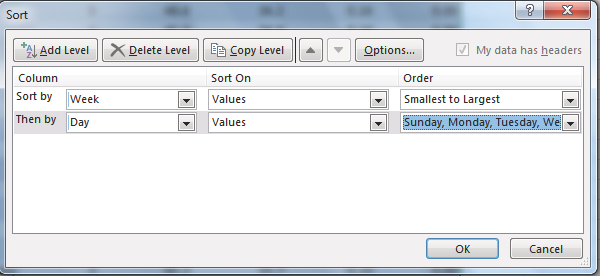
\includegraphics[width=\maxwidth{.95\linewidth}]{gfx/ch05_fig14}
	\caption{Sort Dialog Box}
	\label{05:fig14}
\end{figure}

\begin{enumerate}
	\item Click \fmtButton{OK}.
	\item The sorted table should now look like Figure \ref{05:fig15}. Notice the data is in \textit{Week} order and, within each week, in \textit{Day} order.
%filesave CH5-National Weather
	\item Save the \fmtWorksheet{CH5-National Weather} workbook.
\end{enumerate}

\begin{figure}[H]
	\centering
	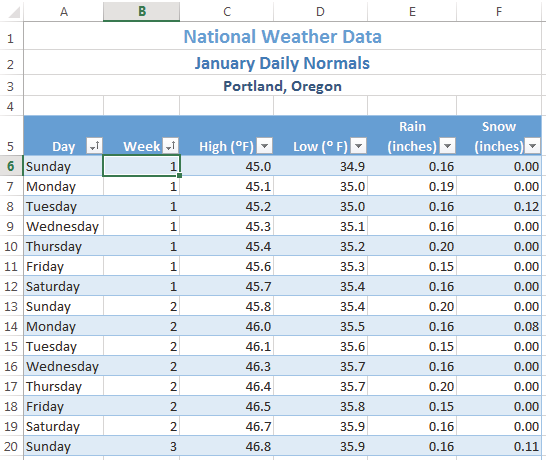
\includegraphics[width=\maxwidth{.95\linewidth}]{gfx/ch05_fig15}
	\caption{Custom Sort}
	\label{05:fig15}
\end{figure}

\begin{center}
	\begin{tkwbox}{Key Take-Aways}
		\textbf{Basic Table Skills}
		\\
		\begin{itemize}
			\setlength{\itemsep}{0pt}
			\setlength{\parskip}{0pt}
			\setlength{\parsep}{0pt}

			\item Tables are made up of adjacent rows and columns of data with a single row of column headings at the top.
			\item Tables are created by clicking in the top left-most cell in the data and clicking \textit{Insert $ \Rightarrow $ Group $ \Rightarrow $ Table}.
			\item There are a gallery of styles and options to choose from to format a table.
			\item To add data it is best to add it one row below the bottom of the table. The table can then be resorted to organize the data.
			\item Freezing heading keeps column headings displayed while scrolling through the table data.
			\item Filter arrows in the table headings sort the data by a single column. Click \textit{Data $ \Rightarrow $ Sort \& Filter $ \Rightarrow $ Sort} to sort by two or more columns at a time.
			\item Custom Sorts can be used when data needs to be sorted in a special way (\ie Days of the Week).
			
		\end{itemize}
	\end{tkwbox}
\end{center}

\section{Advanced Table Skills}

\begin{center}
	\begin{objbox}{Learning Objectives}
		\begin{itemize}
			\setlength{\itemsep}{0pt}
			\setlength{\parskip}{0pt}
			\setlength{\parsep}{0pt}

			\item Filter table data.
			\item Add a total row to a table.
			\item Insert subtotals into a table.
			
		\end{itemize}
	\end{objbox}
\end{center}

\subsection{Filtering Data}

When an Excel table is first created, filter arrows appear in all the column headings. Those arrows can be used to sort the data by a single column. These same arrows can also be used to filter or limit the displayed data within a column. There are many ways to filter data within a column depending on whether the data is text or numeric. 

Notice there is sometimes more than one way to filter data (\ie with a filter choice or a checked box). There are also single criteria filters and multi-criteria filters. As an introduction to filtering, look at just the first week of data in the \textit{Weekly OR} sheet.

\begin{enumerate}
	\item Click on the \fmtWorksheet{Weekly OR} worksheet.
	\item Click cell \fmtLoc{B5}.
	\item Click the filter arrow to the right of the \textit{Week} heading.
	\item Click the \fmtButton{Select All} checkbox to deselect all the checkbox choices.
	\item Click on $ 1 $ to select just Week $ 1 $.
	\item Click \fmtButton{OK}.
\end{enumerate}

The table should look like Figure \ref{05:fig16}. Only seven rows of Week One are visible in the table. Notice in the Status Bar at the bottom of the screen the message ``$ 7 $ of $ 31 $ records found''. Also notice that the filter arrow in the Week heading has changed to a funnel which indicates that this column is currently filtered.

\begin{figure}[H]
	\centering
	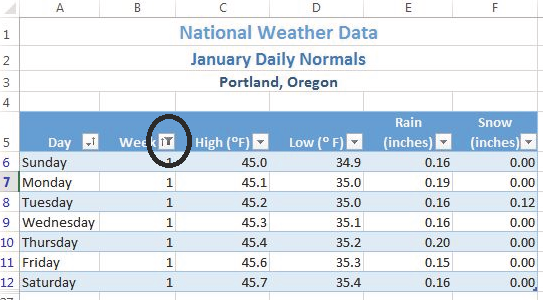
\includegraphics[width=\maxwidth{.95\linewidth}]{gfx/ch05_fig16}
	\caption{Filter}
	\label{05:fig16}
\end{figure}

Follow this procedure to remove the filter.

\begin{enumerate}
	\item Click the funnel next to the Week heading.
	\item Click \fmtButton{Clear Filter from ``Week''}.
\end{enumerate}

\begin{center}
	\begin{sklbox}{Skill Refresher}
		\textbf{Filter a Column}
		\\
		\begin{itemize}
			\setlength{\itemsep}{0pt}
			\setlength{\parskip}{0pt}
			\setlength{\parsep}{0pt}

			\item Click the filter arrow to the right of the heading in the column to be filtered.
			\item Click the \textit{Select All} checkbox to deselect all of the checkbox choices.
			\item Click on the checkboxes to filter by.
			\item Click \textit{OK}.
			
		\end{itemize}
		
		\bigskip
		\textbf{Un-Filter a Column}
		
		\begin{itemize}
			\setlength{\itemsep}{0pt}
			\setlength{\parskip}{0pt}
			\setlength{\parsep}{0pt}
			
			\item Click the funnel to the right of the heading in the column to be filtered.
			\item Select \textit{Clear Filter}.
			
		\end{itemize}
	\end{sklbox}
\end{center}

As an example of using a numeric filter, find the days in Portland ME when it was warmer than $ 32 $ degrees.

\begin{enumerate}
	\item Click in the \fmtWorksheet{Portland ME} worksheet.
	\item Click cell \fmtLoc{B5}.
	\item Click on the filter arrow next to the \textit{High} heading.
	\item Click \fmtButton{Number Filters $ \Rightarrow $ Greater Than...}.
	\item The \textit{Custom AutoFilter} dialog box will appear on the screen.
	\item Enter \fmtTyping{32} in the space to the right of \textit{is Greater than}. The \textit{Custom AutoFilter} dialog box should now match Figure \ref{05:fig17}.
	\item Click \fmtButton{OK}.
\end{enumerate}

\begin{figure}[H]
	\centering
	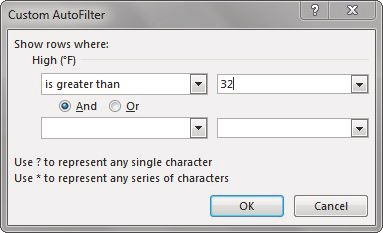
\includegraphics[width=\maxwidth{.95\linewidth}]{gfx/ch05_fig17}
	\caption{AutoFilter Dialog Box}
	\label{05:fig17}
\end{figure}

It is now easy to see that it was above $ 32 $ degrees for only the first three days, as illustrated in Figure \ref{05:fig18}.

\begin{figure}[H]
	\centering
	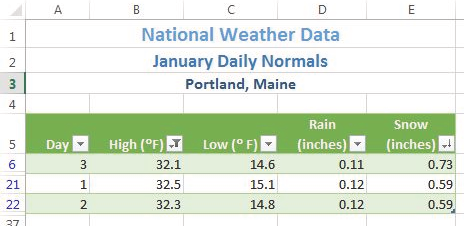
\includegraphics[width=\maxwidth{.95\linewidth}]{gfx/ch05_fig18}
	\caption{Maine Filter Results}
	\label{05:fig18}
\end{figure}

Review sorting and filtering in the following steps.

\begin{enumerate}
	\item Click on the \fmtWorksheet{Weekly OR} worksheet.
	\item Sort the table by \textit{Week} (smallest to largest).
	\item Filter the \textit{Day} to only show \textit{Monday}.
	\item Compare the results to Figure \ref{05:fig19}.
	\item After checking the results, clear the \textit{Day} filter.
\end{enumerate}

\begin{figure}[H]
	\centering
	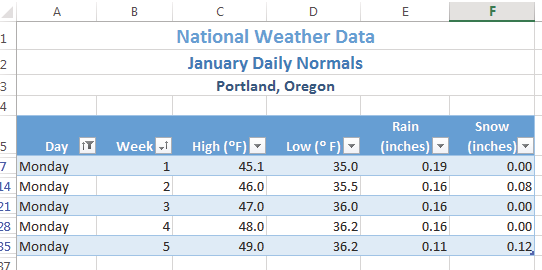
\includegraphics[width=\maxwidth{.95\linewidth}]{gfx/ch05_fig19}
	\caption{Oregon Filter Results}
	\label{05:fig19}
\end{figure}

\subsection{Filtering Using the Slicer}

Beginning in Excel $ 2013 $, slicers were added as another way to filter table data. A slicer is useful because it clearly indicates what data is shown in the table after the data has been filtered.

Try using the Slicer to filter the \textit{Portland OR} data table.

\begin{enumerate}
	\item Click on the \fmtWorksheet{Portland OR} worksheet. 
	\item Click cell \fmtLoc{A5}.
	\item Click \fmtButton{Insert $ \Rightarrow $ Filters $ \Rightarrow $ Slicer}.
	\item Click on \fmtButton{Day} in the \textit{Insert Slicers} dialog box, and then click \fmtButton{OK} (see Figure \ref{05:fig20a}).

	\begin{figure}[H]
		\centering
		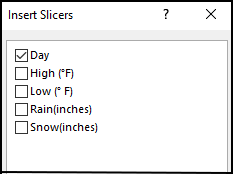
\includegraphics[width=\maxwidth{.50\linewidth}]{gfx/ch05_fig20a}
		\caption{Slicer Dialog Box}
		\label{05:fig20a}
	\end{figure}
	
	\item Drag the slicer box so the top left corner is near the center of cell \fmtLoc{G5}.
	\item Notice that when the Slicer was inserted, a \textit{Slicer Options} tab appears on the ribbon. (\fmtNewExcel{Excel 365}. This tab is named \textit{Slicer} rather than \textit{Slicer Options}.) This tab contains links to change the style and size of the slicer box or individual slicer buttons.
	\item Click \fmtButton{Slicer Tools Options $ \Rightarrow $ Slicer Styles $ \Rightarrow $ Expand Arrow}. The styles illustrated in Figure \ref{05:fig20} will become available.
\end{enumerate}

\begin{figure}[H]
	\centering
	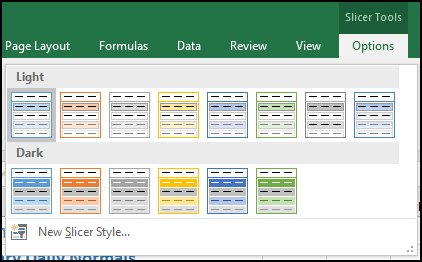
\includegraphics[width=\maxwidth{.95\linewidth}]{gfx/ch05_fig20}
	\caption{Slicer Styles}
	\label{05:fig20}
\end{figure}

\begin{enumerate}
	\item Select the first choice under \textit{Dark}.
	\item Click \fmtButton{Slicer Tools Options $ \Rightarrow $ Size $ \Rightarrow $ Width} and enter \fmtTyping{1} inch. (Note: Do NOT set the size in the \textit{Buttons} group.)
	\item Click in the slicer and scroll down to Day $ 15 $. Click the \fmtButton{15} button to show only the data for day $ 15 $ in the data table.
	\item Click the \textit{Multiselect} button in the top center of the slicer to permit the selection of multiple lines.
	\item Click the Slicer buttons for Days $ 10 $ through $ 14 $. The table should now show the data from Days $ 10-15 $.
	\item Using the filter arrow on the right edge of the \textit{Day} header in \fmtLoc{A5}, sort the column from smallest to largest to show the days in order as in Figure \ref{05:fig21}.
\end{enumerate}

\begin{figure}[H]
	\centering
	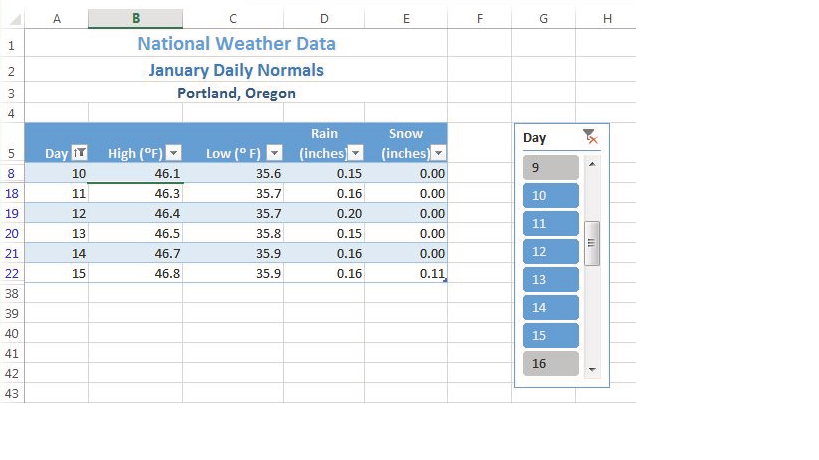
\includegraphics[width=\maxwidth{.95\linewidth}]{gfx/ch05_fig21}
	\caption{Slicer Results}
	\label{05:fig21}
\end{figure}

\begin{enumerate}[resume]
	\item Click the red \fmtButton{X} in the top right corner of the slicer to remove the filter and show the complete data file.
	\item Using the filter arrow on the right edge of the \textit{Day} header in \fmtLoc{A5}, sort the column from smallest to largest to show the days in order.
	\item Click in the top margin of the slicer to select the slicer tool. It should have a thick border and drag handles. Press \fmtKeystroke{Delete} to remove the slicer.
 \end{enumerate}

\subsection{Total Rows}

By adding a total row to the bottom of the table, summary data is easily seen for one or more of the columns. Total rows can be added to tables as a whole or to only those that are filtered. Total rows can easily be toggled on and off as the need for summary data arises.

\begin{enumerate}
	\item Click on the \fmtWorksheet{Portland ME} worksheet.
	\item Clear the filter from the \textit{High} column by clicking the filter down-arrow and then \textit{Clear Filter from High (\textdegree F)}.
	\item Click cell \fmtLoc{A5}.
	\item Click \fmtButton{Table Tools Design $ \Rightarrow $ Table Style Options $ \Rightarrow $ Total Row}. (\fmtNewExcel{Excel 365}. The tab is named \textit{Table Design} rather than \textit{Table Tools Design}.)
	\item Scroll to the bottom of the table to the \textit{Total Row}. Notice the total for the \textit{Snow} data.
	\item Click cell \fmtLoc{D37} (in the \textit{Rain} column), and then click the down-arrow that appears on the right of the cell.
	\item Choose \fmtButton{Sum} to add a sum to the \textit{Total Row} in the \textit{Rain} column.
	\item To see the Average rainfall for the month, click on the arrow again and choose \fmtButton{Average}.
	\item Change the total in cell \fmtLoc{E37} (\textit{Snow}) to see the Average snowfall for the month.
	\item Click \fmtButton{Home $ \Rightarrow $ Number $ \Rightarrow $ Decrease Decimal} to change the decimal places in \fmtLoc{D37} and \fmtLoc{E37} to $ 2 $. Compare the \textit{Total Row} to Figure \ref{05:fig22}.
\end{enumerate}

\begin{figure}[H]
	\centering
	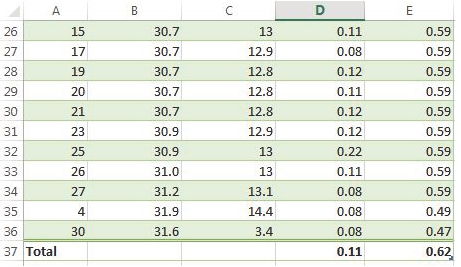
\includegraphics[width=\maxwidth{.95\linewidth}]{gfx/ch05_fig22}
	\caption{Total Row}
	\label{05:fig22}
\end{figure}

Now switch to the \textit{Weekly OR} sheet and add a Slicer and Total Row to this table.

\begin{enumerate}
	\item Open the \fmtWorksheet{Weekly OR} sheet.
	\item If the \textit{Day} column is still filtered, clear it by clicking the filter down-arrow and then clicking the \textit{(Select All)} checkbox.
	\item Add a Slicer for the \textit{Day} column to the sheet.
	\item Drag the slicer so the top left corner is near the center of cell \fmtLoc{H5}. 
	\item Resize the slicer as desired and apply any Slicer Style.
	\item Select Monday through Friday in the Slicer so that Saturday and Sunday data do \textit{NOT} show in the table.
	\item Add a Total Row that averages the \textit{High} and \textit{Low} columns. The averages should be \textit{High}: $ 47.0 $ and \textit{Low}: $ 35.8 $. 
	\item Change the \textit{Total} label to \textit{Average} by clicking cell \fmtLoc{A37} and typing \fmtTyping{Average}.
%filesave CH5-National Weather
	\item Save the \fmtWorksheet{CH5-National Weather} workbook.
\end{enumerate}

\begin{center}
	\begin{sklbox}{Skill Refresher}
		\textbf{Add a Total Row}
		\\
		\begin{itemize}
			\setlength{\itemsep}{0pt}
			\setlength{\parskip}{0pt}
			\setlength{\parsep}{0pt}

			\item Click \textit{Table Tools Design $ \Rightarrow $ Table Style Options $ \Rightarrow $ Total Row}.
			\item Scroll to the bottom of the table to find the Total Row.
			\item Click in one of the columns in the Total Row, and then click the down-arrow that appears to the right of the cell.
			\item Choose \textit{Sum} to add a sum to the Total Row in the column.
			\item To see the Average for column, click on the arrow again and choose \textit{Average}. Some other choices in the Total Row are Count (for words), Count Numbers, Max, and Min.
			
		\end{itemize}
	\end{sklbox}
\end{center}

\begin{center}
	\begin{sklbox}{Skill Refresher}
		\textbf{Add a Slicer}
		\\
		\begin{itemize}
			\setlength{\itemsep}{0pt}
			\setlength{\parskip}{0pt}
			\setlength{\parsep}{0pt}

			\item Click \textit{Insert $ \Rightarrow $ Filters $ \Rightarrow $ Slicer}.
			\item Check the box for the column to which a Slicer is added.
			\item Click \textit{OK}.
			
		\end{itemize}
	\end{sklbox}
\end{center}

\subsection{Subtotaling}

Subtotals and grand totals can be easily calculated for a column in a table. This is a powerful tool that to quickly display multiple levels of summary data within the table. This can provide Management with a report of higher-level summary data one minute, and then can be easily switched back to detailed data the next minute. \textit{It is important to save often during this process and follow the steps carefully.} It is recommended to make a copy of the data to be subtotaled and place it in a new sheet, so the summary subtotaled data can be separately saved if desired.

The following steps summarize the process to add subtotals to a worksheet.

\begin{enumerate}
	\item Sort by the column to subtotal on.
	\item Convert the table back to a normal Excel range since a table cannot contain a subtotal.
	\item Click \textit{Data $ \Rightarrow $ Outline $ \Rightarrow $ Subtotal}.
	\item To limit the displayed data further, click \textit{Data $ \Rightarrow $ Sort \& Filter $ \Rightarrow $ Filter}.
\end{enumerate}

To practice subtotaling, determine what the weather looks like for each day of the week.

\begin{enumerate}
	\item Click on the \fmtWorksheet{Weekly OR} sheet.
	\item Hover the mouse over the \fmtWorksheet{Weekly OR} sheet tab at the bottom of the screen, hold the \fmtKeystroke{Ctrl} key down and then click-and-drag the sheet to the right until it is past all the existing sheets.
	\item When a sheet icon with a \textbf{+} sign is visible, let go of the mouse button and then the \fmtKeystroke{Ctrl} key. A \fmtWorksheet{Weekly OR (2)} sheet will appear.
	\item Right-click on the new sheet tab, select \fmtButton{Rename}, type \fmtTyping{Subtotal OR}, and then press \fmtKeystroke{Enter}.
%filesave CH5-National Weather
	\item Save the \fmtWorksheet{CH5-National Weather} workbook.
	\item Remove all filters in the table by clicking \fmtButton{Data $ \Rightarrow $ Sort \& Filter $ \Rightarrow $ Clear}.
	\item Click in the top margin of the slicer to select the slicer tool. It should have a thick border and drag handles. Press \fmtKeystroke{Delete} to remove the slicer.

	\item Click \fmtButton{Data $ \Rightarrow $ Sort \& Filter $ \Rightarrow $ Sort}. 
	\item Click the down-arrow for \textit{Column Sort By} and select \textit{Day}.
	\item Click the down-arrow for \textit{Order} and select \textit{Custom List}.
	\item Select the custom list Sunday, Monday, Tuesday, etc. (See Figure \ref{05:fig13} through Figure \ref{05:fig15} for a review of Custom Sorting.)
	\item Click \fmtButton{OK} then click \fmtButton{OK} a second time.
	\item Before adding subtotals, convert the table back to a regular range. To do this, click \fmtButton{Table Tools Design $ \Rightarrow $ Tools $ \Rightarrow $ Convert to Range} (see Figure \ref{05:fig23}). (\fmtNewExcel{Excel 365}. This tab is called \textit{Table Design} rather than \textit{Table Tools Design}.)
\end{enumerate}

\begin{figure}[H]
	\centering
	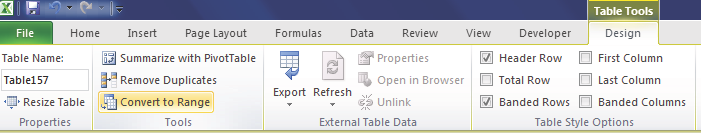
\includegraphics[width=\maxwidth{.95\linewidth}]{gfx/ch05_fig23}
	\caption{Convert to Range}
	\label{05:fig23}
\end{figure}

\begin{enumerate}[resume]
	\item When a box pops up with a warning about converting the table, click \fmtButton{Yes}.
	\item Click cell \fmtLoc{A6}.
	\item Click \fmtButton{Data $ \Rightarrow $ Outline $ \Rightarrow $ Subtotal}.
	\item In the \textit{Subtotal Window}, make the choices shown in the Figure \ref{05:fig24}. It is essential to select the column that the data is sorted by in the \textit{At each change in field} at the top of the window. 
	\item Click \fmtButton{OK}.
\end{enumerate}

\begin{figure}[H]
	\centering
	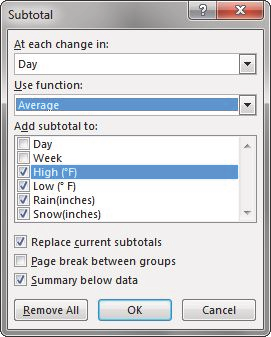
\includegraphics[width=\maxwidth{.95\linewidth}]{gfx/ch05_fig24}
	\caption{Subtotal Window}
	\label{05:fig24}
\end{figure}

The data should look like Figure \ref{05:fig25}. Successful subtotaling shows only one subtotal for each group in the column sorted by. (\textit{HINT}: If there is more than one Subtotal for the same group (\ie one of the days of the week in the example), then the column was not sorted before subtotaling. Remove the subtotals using the \textit{Remove All} button in Figure \ref{05:fig24}, sort the table, and then subtotal again.)

\begin{figure}[H]
	\centering
	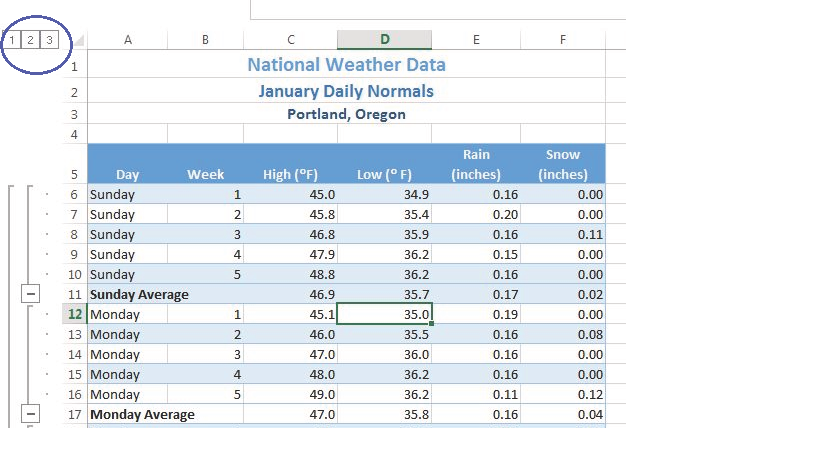
\includegraphics[width=\maxwidth{.95\linewidth}]{gfx/ch05_fig25}
	\caption{Subtotal Results}
	\label{05:fig25}
\end{figure}

Notice the three \textit{Outline} buttons circled in the upper-left corner of the spreadsheet. These control the amount of subtotaled data that is displayed. Table \ref{05:tab06} describes the different \textit{Outline} buttons.

\begin{table}[H]
	\rowcolors{1}{}{tablerow} % zebra striping background
	{\small
		%\fontsize{8}{10} \selectfont %Replace small for special font size
		\begin{longtable}{L{0.50in}L{3.00in}} %Left-aligned, Max width: 4.25in
			\textbf{Button} & \textbf{Content Displayed} \endhead
			\hline
			Level 1 & Only the grand average\\
			Level 2 & Subtotals and grand total\\
			Level 3 & Individual records, subtotals, and grand total\\
			\rowcolor{captionwhite}
			\caption{Subtotal Outline Buttons}
			\label{05:tab06}
		\end{longtable}
	} % End small
\end{table}

Click the three \textit{Outline} buttons to see the difference in the data displayed.

\begin{enumerate}
	\item Click on the \fmtButton{$ 1 $ Outline} button in the upper left-hand corner of the sheet.
	\item Only the \textit{Grand Average} row with averages for High, Low, Rain, and Snow should be visible.
	\item Click on the \fmtButton{$ 2 $ Outline} button.
	\item The average for each day of the week along with the \textit{Grand Average} are now visible.
	\item Click on the \fmtButton{+ Sign} button to the left of the Sunday Average row.
	\item This expands just the \textit{Sunday Day} data and displays the individual records for this subset of the data. Clicking on \fmtButton{+ Sign} buttons will expand a portion of the data at a time. Clicking on \fmtButton{– Sign} buttons hide a portion of the data at a time.
	\item Click on the \fmtButton{$ 3 $ Outline} button.
	\item All the individual records along with the subtotals, and \textit{Grand Average} should be displayed. 
%filesave CH5-National Weather
	\item Save the \fmtWorksheet{CH5-National Weather} workbook.
\end{enumerate}

\begin{center}
	\begin{tkwbox}{Key Take-Aways}
		\textbf{Advanced Table Skills}
		\\
		\begin{itemize}
			\setlength{\itemsep}{0pt}
			\setlength{\parskip}{0pt}
			\setlength{\parsep}{0pt}

			\item Filtering is an easy way to see a subset of the data. Filtering arrows appear to the right of each column heading when the table has a header row.
			\item Data can be filtered by text or numerically.
			\item A slicer is another way to filter in Excel that provides a set of filtering buttons on the sheet.
			\item Adding a total row to a table is a quick, efficient way to see summary statistics for one or more columns in a table.
			\item Subtotaling provides a way to quickly add totals to groups within a column along with providing a grand total at the bottom of the table.
			\item Subtotal Outline buttons allow users to see add of the subtotaled data, just the totals and grand total, or simply the grand total.
			\item $ + $ and $ - $ buttons within subtotaling allow a user to expand and hide portions of the subtotaled data.
			
		\end{itemize}
	\end{tkwbox}
\end{center}

\section{Preparing to Print}

\begin{center}
	\begin{objbox}{Learning Objectives}
		\begin{itemize}
			\setlength{\itemsep}{0pt}
			\setlength{\parskip}{0pt}
			\setlength{\parsep}{0pt}

			\item Review options for professional page setup for printing.
			\item Understand how to insert a picture to enhance the visual appearance of a worksheet.
			\item Preview worksheets containing tables to ensure they will print in a professional manner.
			
		\end{itemize}
	\end{objbox}
\end{center}

\subsection{Previewing a Worksheet}

Now that the weather data has been sorted, filtered, and subtotaled as needed, it is time to print the worksheets. Start with the \textit{Portland ME} worksheet.

\begin{enumerate}
	\item Click on the \fmtWorksheet{Portland ME} worksheet. 
	\item Click cell \fmtLoc{A1}.
\end{enumerate}

Notice that cells $ A1 $, $ A2 $, and $ A3 $ are not merged and centered over the entire width of the table. 

\begin{enumerate}
	\item Select cell \fmtLoc{A1} and click \fmtButton{Home $ \Rightarrow $ Alignment $ \Rightarrow $ Merge \& Center}. This should split \fmtLoc{A1} into four cells (\fmtLoc{A1:D1}).
	\item Select the range \fmtLoc{A1:E1} and click \fmtButton{Home $ \Rightarrow $ Alignment $ \Rightarrow $ Merge \& Center}. Cell \fmtLoc{A1} should now be merged across \fmtLoc{A1:E1}.
	\item Repeat these steps for \fmtLoc{A2} and \fmtLoc{A3}.
\end{enumerate}

Next, open \textit{Print Preview} and determine what page setup options need to be set.

\begin{enumerate}
	\item Click \fmtButton{File $ \Rightarrow $ Print}.
	\item Notice that the table should be centered on the page.
	\item At the bottom of the \textit{Settings} section, click the link for \fmtButton{Page Setup}. This opens the \textit{Page Setup} dialog box. 
	\item Click on the \fmtButton{Margins} tab. See Figure \ref{05:fig26}.
\end{enumerate}

\begin{figure}[H]
	\centering
	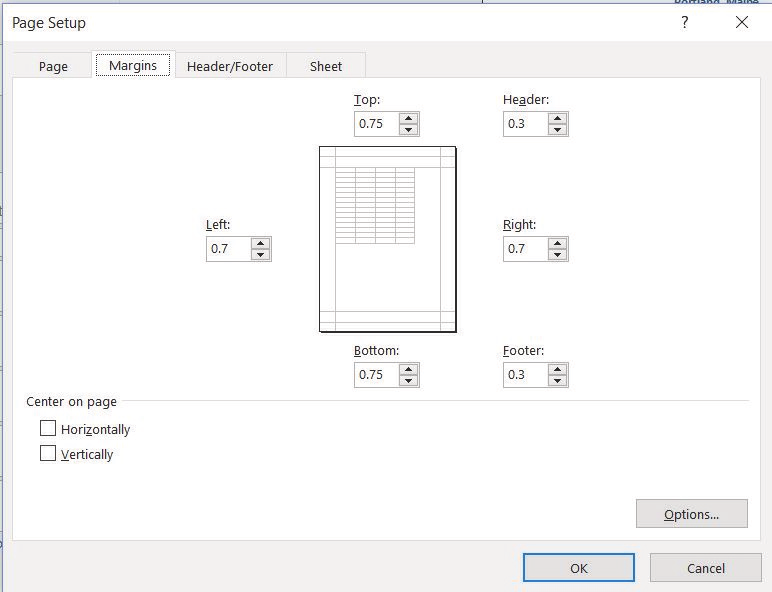
\includegraphics[width=\maxwidth{.95\linewidth}]{gfx/ch05_fig26}
	\caption{Page Setup}
	\label{05:fig26}
\end{figure}

\begin{enumerate}[resume]
	\item In the \textit{Center on page} section, check the box for \fmtButton{Horizontally}.
	\item Click \fmtButton{OK}. The table should now be centered horizontally on the page.
	\item Next, add a footer with the workbook filename and worksheet name.
	\item At the bottom of the \textit{Print Preview Settings} section, click the link for \fmtButton{Page Setup}. This opens the \textit{Page Setup} dialog box.	
	\item Click the \fmtButton{Header/Footer} tab then click the \fmtButton{Custom Footer} button.
	\item In the \textit{Left section:} box type \fmtTyping{File:} (making sure to leave a space after the colon).
	\item Click the \fmtButton{Insert File Name} button (see Figure \ref{05:fig26a}).
	\item In the \textit{Right section:} box type \fmtTyping{Worksheet:} (making sure to leave a space after the colon).
	\item Click the \fmtButton{Insert Sheet Name} button.
	
	\begin{figure}[H]
		\centering
		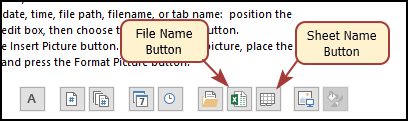
\includegraphics[width=\maxwidth{.85\linewidth}]{gfx/ch05_fig26a}
		\caption{File/Sheet Name Button Locations}
		\label{05:fig26a}
	\end{figure}
		
	\item The completed Footer dialog box should look like Figure \ref{05:fig27}. Click the \fmtButton{OK} button twice to return to \textit{Print Preview}. 
	\item Confirm that the footer appears correctly, then click the arrow at the top left corner of the screen to exit \textit{Print Preview}.
\end{enumerate}

\begin{figure}[H]
	\centering
	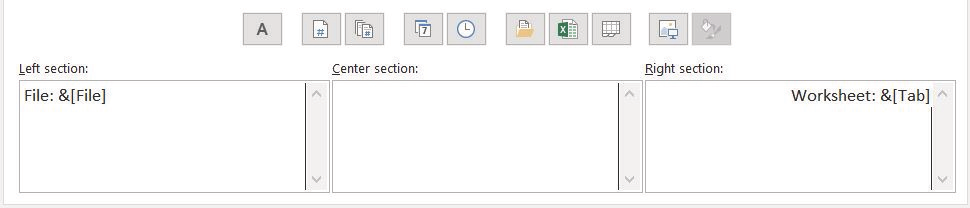
\includegraphics[width=\maxwidth{.95\linewidth}]{gfx/ch05_fig27}
	\caption{Custom Footer}
	\label{05:fig27}
\end{figure}

\subsection{Inserting an Image to Enhance a Worksheet}

Next add a small weather-related graphic to the worksheet to enhance its appearance. In Excel, an image file from either the local hard drive or downloaded from an online source can be used. For this exercise, use the graphic in the student files for this chapter.

\begin{enumerate}
	\item \fmtOldExcel{Excel 2016} Click \fmtButton{Insert $ \Rightarrow $ Illustrations $ \Rightarrow $ Pictures}. (This inserts an image from the local computer. To search for an online image, click the \fmtButton{Online Pictures} button.) (See Figure \ref{05:fig28}.)
	\item \fmtNewExcel{Excel 365} Click \fmtButton{Insert $ \Rightarrow $ Illustrations $ \Rightarrow $ Pictures $ \Rightarrow $ This Device}. (This inserts an image from the local computer. To search for an online image, click the \fmtButton{Online Pictures} button in the \textit{Pictures} dropdown menu.)
\end{enumerate}

\begin{figure}[H]
	\centering
	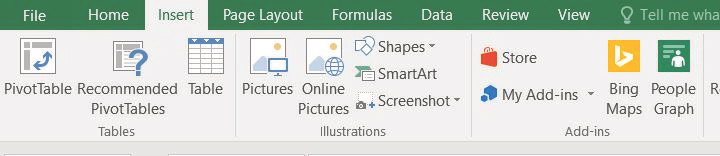
\includegraphics[width=\maxwidth{.95\linewidth}]{gfx/ch05_fig28}
	\caption{Insert Pictures}
	\label{05:fig28}
\end{figure}

\begin{enumerate}[resume]
	\item Navigate to the folder containing the Chapter $ 5 $ files and double-click the \textit{CH5-Weather.png} image file.
\end{enumerate}

The image now appears on the worksheet, but not in the desired location. It is also slightly larger than desired (see Figure \ref{05:fig29}).

\begin{figure}[H]
	\centering
	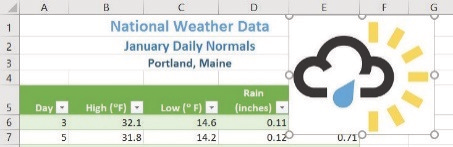
\includegraphics[width=\maxwidth{.95\linewidth}]{gfx/ch05_fig29}
	\caption{Inserted Image}
	\label{05:fig29}
\end{figure}

\begin{enumerate}
	\item Place the mouse pointer in the image so that the pointer changes to crosshairs. Drag the image so that the top left corner is at the left edge of cell \fmtLoc{E1}.
	\item Using the resizing handle in the bottom right corner of the image, resize the image so that it does not cover any of the table. Hint: drag diagonally to the left and up. The bottom right corner of the image will end up near the left edge of cell \fmtLoc{F4}.
	\item Check \textit{Print Preview} again to make sure the worksheet with the image added looks good.
	\item Exit \textit{Print Preview}.
%filesave CH5-National Weather
	\item Save the \fmtWorksheet{CH5-National Weather} workbook.
\end{enumerate}

\subsection{Previewing the Remaining Worksheets}

Before considering this workbook finished, confirm that the remaining worksheets are all printing appropriately.

\begin{enumerate}
	\item Click the \fmtWorksheet{Portland OR} worksheet.
	\item Click \fmtButton{File $ \Rightarrow $ Print}.
	\item No changes need to be made to this worksheet so click the arrow in the top left corner of the screen to exit \textit{Print Preview}.

	\item Click the \fmtWorksheet{Weekly OR} worksheet.
	\item Click \fmtButton{File $ \Rightarrow $ Print}.
	\item Notice that the Slicer is printing on a second page. To fix this, set the \textit{Page Scaling} to \fmtButton{Fit All Columns on One Page}.
	\item If one or more Slicer buttons are cut off, exit \textit{Print Preview}, and resize the Slicer so that all of the buttons display then return to \textit{Print Preview}.
	\item Confirm the worksheet, including the slicer, is printing appropriately. 
	\item Click the arrow in the top left corner of the screen to exit \textit{Print Preview}.

	\item Click the \fmtWorksheet{Subtotal OR} worksheet.
	\item Click \fmtButton{File $ \Rightarrow $ Print}.
	\item Click \fmtButton{Page Setup} at the bottom of the \textit{Settings} area.
	\item Center this worksheet horizontally on the page. 
	\item Click the arrow in the top left corner of the screen to exit \textit{Print Preview}.

%filesave CH5-National Weather
	\item Save the \fmtWorksheet{CH5-National Weather} workbook.
%fileclose CH5-National Weather
	\item Compare the worksheet with the self-check answer key (\fmtWorksheet{CH5-National Weather Solution}) and then close and submit the \fmtWorksheet{CH5-National Weather} workbook as directed by the instructor.
\end{enumerate}

\begin{center}
	\begin{tkwbox}{Key Take-Aways}
		\textbf{Printing}
		\\
		\begin{itemize}
			\setlength{\itemsep}{0pt}
			\setlength{\parskip}{0pt}
			\setlength{\parsep}{0pt}

			\item When working with Excel workbooks, the final step should always be to review the worksheets in \textit{Print Preview} to make sure they are printing appropriately.
			\item Images can be added to a worksheet to enhance its appearance. Be sure to resize and move them appropriately so they do not detract from the data.

		\end{itemize}
	\end{tkwbox}
\end{center}

\section{Chapter Practice}

\subsection{Tables for a Tourism Company}

\begin{figure}[H]
	\centering
	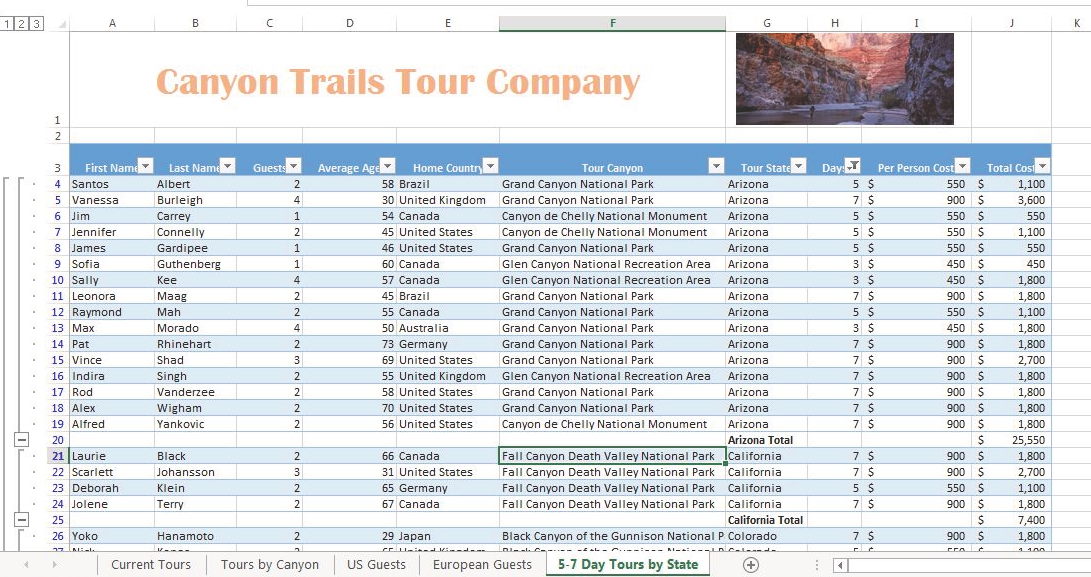
\includegraphics[width=\maxwidth{.95\linewidth}]{gfx/ch05_fig30}
	\caption{Chapter Practice Completed Exercise}
	\label{05:fig30}
\end{figure}

Travel and tour companies need to keep track of client data as well as travel/tour options and tour guides. Keeping up-to-date, accurate records is essential to their bottom line. To run a tour company, employees must be able to manipulate their data quickly and easily. This exercise illustrates how to use the skills presented in this chapter to generate the data needed daily by a tourism company. Figure \ref{05:fig30} shows one of the completed worksheets.

\begin{enumerate}
%fileopen PR5-Data
%filesave PR5-Canyon Trails
	\item Open the data file \fmtWorksheet{PR5-Data} and save the file as \fmtWorksheet{PR5-Canyon Trails}.
	\item In \fmtLoc{J4}, calculate \textit{Total Cost} (\fmtTyping{Guests*Per Person Cost}). Copy the formula down the column.
	\item Format \fmtLoc{Column I} and \fmtLoc{Column J} as \textit{Accounting} with no decimal places.
	\item Center all headings in \fmtLoc{Row }$ 3 $.
	\item Click cell \fmtLoc{A3}. Insert a table with headers for the range \fmtLoc{A3:J53}.
	\item Adjust column widths within the table so that all the headings are completely visible.
	\item Rename \fmtWorksheet{Sheet $ 1 $} to \fmtTyping{Current Tours}. Sort this sheet alphabetically (A to Z) by \textit{Last Name}.

	\item Make a copy of the \fmtWorksheet{Current Tours} sheet and rename it \fmtWorksheet{Tours by Canyon}.
	\item Place the \fmtWorksheet{Tours by Canyon} sheet to the right of the \fmtWorksheet{Current Tours} sheet.
	\item Sort the \fmtWorksheet{Tours by Canyon} worksheet by \textit{Tour Canyon} (A to Z), then \textit{Home Country} (A to Z), and then \textit{Last Name} (A to Z).

	\item Make another copy of the \fmtWorksheet{Current Tours} sheet and rename it \fmtWorksheet{US Guests}.
	\item Place the \fmtWorksheet{US Guests} sheet to the right of the \fmtWorksheet{Tours by Canyon} sheet.
	\item Filter the \fmtWorksheet{US Guests} worksheet so that only guests with a \textit{Home Country} of the United States show. 
	\item Sort the worksheet by \textit{Tour State} (A to Z).
	\item Add a Total Row that sums the \textit{Guests} and \textit{Total Cost} columns.

	\item Make another copy of the \fmtWorksheet{Current Tours} sheet and rename it \fmtWorksheet{European Guests}. 
	\item Place the \fmtWorksheet{European Guests} sheet to the right of the \fmtWorksheet{US Guests} sheet. 
	\item On the \fmtWorksheet{European Guests} worksheet, hide the \textit{Average Age} column.
	\item Insert a slicer in the \fmtWorksheet{European Guests} sheet for \textit{Home Country}. Move the slicer so its top left corner is near the center of \fmtLoc{K3}. Click-and-drag the bottom right corner of the slicer so it is near the center of \fmtLoc{N16}.
	\item Select both \textit{Germany} and the \textit{United Kingdom} on the slicer.
	\item Sort the filtered sheet by \textit{Home Country} (A to Z) and then \textit{Last Name} (A to Z).

	\item Make one more copy of the \fmtWorksheet{Current Tours} sheet and rename it \fmtWorksheet{Tours by State}.
	\item Place the \fmtWorksheet{Tours by State} sheet to the right of the \fmtWorksheet{European Guests} sheet. 
	\item Subtotal the sheet by \textit{Tour State}, summing the \textit{Total Cost} column. (Remember to sort the worksheet by \textit{Tour State} before applying subtotals.)
	\item Change the name of the \fmtWorksheet{Tours by State} sheet to \fmtWorksheet{$ 5-7 $ Day Tours by State}. Filter out $ 3 $-day tours in the table.
%filesave PR5-Canyon Trails
	\item Save the \fmtWorksheet{PR5-Canyon Trails} workbook.
	\item On each worksheet, make the following print setup changes.

	\begin{enumerate}
		\item Add a footer with the worksheet name in the center.
		\item Change to \fmtButton{Landscape Orientation}.
		\item Set the scaling to \fmtButton{Fit All Columns on One Page}.
	\end{enumerate}

	\item For any worksheets that print on more than one page, add Print Titles to repeat the first three rows at the top of each page.
	\item Make sure the sheets are in the following order from left to right: \fmtWorksheet{Current Tours}, \fmtWorksheet{Tours by Canyon}, \fmtWorksheet{US Guests}, \fmtWorksheet{European Guests}, and \fmtWorksheet{$ 5-7 $ Day Tours by State}.
%filesave PR5-Canyon Trails
	\item Save the \fmtWorksheet{PR5-Canyon Trails} workbook.
%fileclose PR5-Canyon Trails
%filesolution PR5-Canyon Trails Solution
	\item Compare the workbook with the self-check answer key (\fmtWorksheet{PR5-Canyon Trails Solution}) and then close and submit the \fmtWorksheet{PR5-Canyon Trails} workbook as directed by the instructor.

\end{enumerate}

\section{Scored Assessment}

\subsection{Tables for a Retail Company}

Retail companies with online and in-store sales have a huge quantity of data to keep track of. Keeping track of sales, costs, and profits on a daily basis is essential to making the most of a business. This exercise illustrates how to use the skills presented in this chapter to generate the data needed on a daily basis by a retail company. Figure \ref{05:fig31} shows the completed worksheet.

\begin{figure}[H]
	\centering
	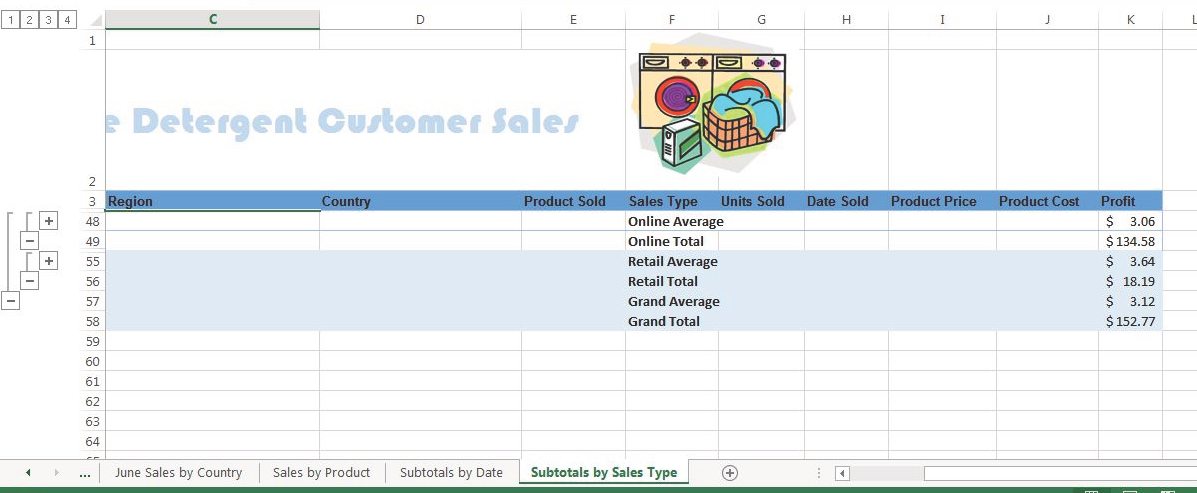
\includegraphics[width=\maxwidth{.95\linewidth}]{gfx/ch05_fig31}
	\caption{Scored Assessment Completed Exercise}
	\label{05:fig31}
\end{figure}

\begin{enumerate}
%fileopen SC5-Data
%filesave SC5-Dynamite Customer Sales
	\item Open \fmtWorksheet{SC5-Data} and save the file as \fmtWorksheet{SC5-Dynamite Customer Sales}.
	\item Click on the \fmtWorksheet{Sales} worksheet.
	\item In \fmtLoc{I4}, enter a \fmtTyping{Vlookup} function that will find the \textit{Product Price} for the Product in \fmtLoc{E4} using the table in the \fmtWorksheet{Product Table} worksheet. In the \fmtTyping{Vlookup} function, fill in the required parameters using the values below along with Figure \ref{05:fig32} as a reference. (Notice that the \textit{Table\_array} parameter uses absolute cell references.)
	
	\begin{itemize}
		\item \textbf{Lookup\_value}: E$ 4 $
		\item \textbf{Table\_array}: 'Product Table'!\$A\$$ 1 $:\$D\$$ 13 $
		\item \textbf{Col\_index\_num}: $ 4 $
		\item \textbf{Range\_lookup}: False
	\end{itemize}
	
\end{enumerate}

\begin{figure}[H]
	\centering
	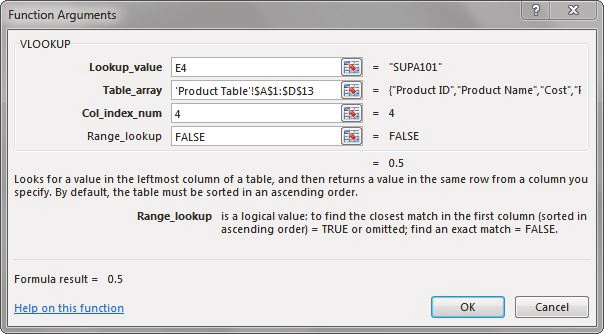
\includegraphics[width=\maxwidth{.95\linewidth}]{gfx/ch05_fig32}
	\caption{\fmtTyping{Vlookup} window}
	\label{05:fig32}
\end{figure}

\begin{enumerate}[resume]
	\item Copy cell \fmtLoc{I5} to \fmtLoc{I6:I52}. 
	\item In \fmtLoc{J4}, enter a \fmtTyping{Vlookup} function that will find the \textit{Product Cost} for the \textit{Product} in \fmtLoc{E4} using the table in the \fmtWorksheet{Product Table} worksheet. Note that the COL\_INDEX\_NUM needs to be $ 3 $ instead of $ 4 $. 
	\item Copy \fmtLoc{J4} to \fmtLoc{J5:J52}.
	\item In \fmtLoc{K4}, calculate \textit{Profit} (\textit{Product Price} $ – $ \textit{Product Cost}).
	\item Copy \fmtLoc{K4} to \fmtLoc{K5:K52}.
	\item Format \fmtLoc{Columns I}, \fmtLoc{Column J}, and \fmtLoc{Column K} as \textit{Accounting} with two decimal places.
	\item Click cell \fmtLoc{A3}. Insert a table with headers for the range \fmtLoc{A3:K52}. \textit{BE CAREFUL HERE}: Excel will try to insert a table starting with \fmtLoc{A2}. Be certain the range starts with \fmtLoc{A3}.
\end{enumerate}

\noindent
\textbf{Online Sales by Date}

\begin{enumerate}[resume]
	\item Make a copy of the \fmtWorksheet{Sales} sheet.
	\item Rename \fmtWorksheet{Sales (2)} to \fmtWorksheet{Online Sales by Date}. \item Place \fmtWorksheet{Online Sales by Date} to the right of the \fmtWorksheet{Sales} worksheet. 
	\item On the \fmtWorksheet{Online Sales by Date} worksheet, filter \textit{Sales Type} so that only \textit{Online Sales} are displayed. 
	\item Sort the filtered data by \textit{Date Sold} (Oldest to Newest).
\end{enumerate}

\noindent
\textbf{June Sales by Country}

\begin{enumerate}[resume]
	\item Make a copy of the \fmtWorksheet{Sales} sheet and rename it \fmtWorksheet{June Sales by Country}. 
	\item Place \fmtWorksheet{June Sales by Country} to the right of the \fmtWorksheet{Online Sales by Date} worksheet. 
	\item On the \fmtWorksheet{June Sales by Country} worksheet, filter \textit{Date Sold} to only show \textit{June} dates by using the \textit{Date Filter Between}. 
	\item Sort the worksheet by \textit{Country} (A to Z) and then by \textit{Name} (A to Z).
\end{enumerate}

\noindent
\textbf{Sales by Product}

\begin{enumerate}[resume]
	\item Make another copy of the \fmtWorksheet{Sales} sheet and rename it \fmtWorksheet{Sales by Product}. 
	\item Place \fmtWorksheet{Sales by Product} to the right of the \fmtWorksheet{June Sales by Country} worksheet. 
	\item In the \fmtWorksheet{Sales by Product} worksheet, hide the \textit{Region} column.
	\item Insert a slicer for \textit{Product Sold}. Move the slicer so its top left corner is near the center of \fmtLoc{L3}. Click-and-drag the bottom right corner of the slicer so it is near the center of \fmtLoc{O16}.
	\item Select both \textit{DETA100} and \textit{DETA200} in the slicer (all other products should be off). 
	\item Sort the filtered sheet by \textit{Product Sold} (A to Z). 
	\item Add a \textit{Total Row} that includes the average for the \textit{Product Price}, \textit{Product Cost}, and \textit{Profit} columns. 
	\item Change the heading in \fmtLoc{A53} to \fmtTyping{Average}.
\end{enumerate}

\noindent
\textbf{Subtotals by Date}

\begin{enumerate}[resume]
	\item Make a copy of the \fmtWorksheet{Sales} sheet and rename it \fmtWorksheet{Subtotals by Date}. 
	\item Place \fmtWorksheet{Subtotals by Date} to the right of the \fmtWorksheet{Sales by Product} worksheet. 
	\item In the \fmtWorksheet{Subtotals by Date} worksheet, subtotal the sheet by \textit{Date Sold} (Oldest to Newest), summing the \textit{Profit} column. 
	\item Click the \fmtButton{2 Outline} button to show just the subtotals by date and the Grand Total.
\end{enumerate}

\noindent
\textbf{Subtotals by Type}

\begin{enumerate}[resume]
	\item Make a copy of the \fmtWorksheet{Sales} sheet and rename it \fmtWorksheet{Subtotals by Type}. 
	\item Place \fmtWorksheet{Subtotals by Type} to the right of the \fmtWorksheet{Subtotals by Date} worksheet. 
	\item Subtotal the sheet by \textit{Sales Type}, summing the \textit{Profit} column.
	\item Add a second subtotal that subtotals by \textit{Type} and averages the \textit{Profit} column. (\textit{Hint}: uncheck \fmtButton{Replace Current Subtotals} in the \textit{Subtotal} dialog box.) 
	\item Notice that four outline buttons appear with the second subtotal. Experiment to determine which outline button to click to display the \textit{Average} and \textit{Total} subtotals for both \textit{Online} and \textit{Retail} along with the \textit{Grand Average} and \textit{Grand Total}.
\end{enumerate}

\noindent
\textbf{Print Settings}

\begin{enumerate}[resume]
	\item For each worksheet, click \fmtButton{Insert $ \Rightarrow $ Text $ \Rightarrow $ Header \& Footer} to add a custom footer with the worksheet name in the center.
	\item Preview each worksheet in \textit{Print Preview} and make any necessary changes for professional printing. (\textit{Hint}: Orientation, page scaling, and print titles might need to be adjusted.)
	\item Double-check that the sheets are in the following order from left to right: \fmtWorksheet{Sales}, \fmtWorksheet{Online Sales by Date}, \fmtWorksheet{June Sales by Country}, \fmtWorksheet{Sales by Product}, \fmtWorksheet{Subtotals by Date}, \fmtWorksheet{Subtotals by Type}, and \fmtWorksheet{Product Table}.
%filesave SC5-Dynamite Customer Sales
%fileclose SC5-Dynamite Customer Sales
	\item Save and close the \fmtWorksheet{SC5-Dynamite Customer Sales} workbook.
	\item Submit the \fmtWorksheet{SC5-Dynamite Customer Sales} workbook as directed by the instructor.
\end{enumerate}
